%HOLASDASDA




\documentclass{beamer}\usepackage{graphicx, color}
%% maxwidth is the original width if it is less than linewidth
%% otherwise use linewidth (to make sure the graphics do not exceed the margin)
\makeatletter
\def\maxwidth{ %
  \ifdim\Gin@nat@width>\linewidth
    \linewidth
  \else
    \Gin@nat@width
  \fi
}
\makeatother

\definecolor{fgcolor}{rgb}{0.2, 0.2, 0.2}
\newcommand{\hlnumber}[1]{\textcolor[rgb]{0,0,0}{#1}}%
\newcommand{\hlfunctioncall}[1]{\textcolor[rgb]{0.501960784313725,0,0.329411764705882}{\textbf{#1}}}%
\newcommand{\hlstring}[1]{\textcolor[rgb]{0.6,0.6,1}{#1}}%
\newcommand{\hlkeyword}[1]{\textcolor[rgb]{0,0,0}{\textbf{#1}}}%
\newcommand{\hlargument}[1]{\textcolor[rgb]{0.690196078431373,0.250980392156863,0.0196078431372549}{#1}}%
\newcommand{\hlcomment}[1]{\textcolor[rgb]{0.180392156862745,0.6,0.341176470588235}{#1}}%
\newcommand{\hlroxygencomment}[1]{\textcolor[rgb]{0.43921568627451,0.47843137254902,0.701960784313725}{#1}}%
\newcommand{\hlformalargs}[1]{\textcolor[rgb]{0.690196078431373,0.250980392156863,0.0196078431372549}{#1}}%
\newcommand{\hleqformalargs}[1]{\textcolor[rgb]{0.690196078431373,0.250980392156863,0.0196078431372549}{#1}}%
\newcommand{\hlassignement}[1]{\textcolor[rgb]{0,0,0}{\textbf{#1}}}%
\newcommand{\hlpackage}[1]{\textcolor[rgb]{0.588235294117647,0.709803921568627,0.145098039215686}{#1}}%
\newcommand{\hlslot}[1]{\textit{#1}}%
\newcommand{\hlsymbol}[1]{\textcolor[rgb]{0,0,0}{#1}}%
\newcommand{\hlprompt}[1]{\textcolor[rgb]{0.2,0.2,0.2}{#1}}%

\usepackage{framed}
\makeatletter
\newenvironment{kframe}{%
 \def\at@end@of@kframe{}%
 \ifinner\ifhmode%
  \def\at@end@of@kframe{\end{minipage}}%
  \begin{minipage}{\columnwidth}%
 \fi\fi%
 \def\FrameCommand##1{\hskip\@totalleftmargin \hskip-\fboxsep
 \colorbox{shadecolor}{##1}\hskip-\fboxsep
     % There is no \\@totalrightmargin, so:
     \hskip-\linewidth \hskip-\@totalleftmargin \hskip\columnwidth}%
 \MakeFramed {\advance\hsize-\width
   \@totalleftmargin\z@ \linewidth\hsize
   \@setminipage}}%
 {\par\unskip\endMakeFramed%
 \at@end@of@kframe}
\makeatother

\definecolor{shadecolor}{rgb}{.97, .97, .97}
\definecolor{messagecolor}{rgb}{0, 0, 0}
\definecolor{warningcolor}{rgb}{1, 0, 1}
\definecolor{errorcolor}{rgb}{1, 0, 0}
\newenvironment{knitrout}{}{} % an empty environment to be redefined in TeX

\usepackage{alltt}

\usetheme{Warsaw}
\usepackage[buttonsize=1em]{animate}
%\hypersetup{urlcolor=blue}

\title[useRChile]{Presentando rgexf + tips para armar tu propio paquete}
\author[GGV]{George G. Vega (george.vega@nodoschile.org)}
\institute[useRchile]{Grupo de Usuarios de R en Chile}
\date{15 de junio, 2013}

\titlegraphic{
\includegraphics[width=2cm]{../../imagenes/usaR}\hspace*{4.75cm}~%
   
\includegraphics[width=2cm]{../../imagenes/RevolutionAnalyics}
}
\IfFileExists{upquote.sty}{\usepackage{upquote}}{}

\begin{document}

\begin{frame}
\maketitle
\end{frame}

\begin{frame}

\frametitle{Agenda}
\tableofcontents
\end{frame}

%%%%%%%%%%%%%%%%%%%%%%%%%%%%%%%%%%%%%%%%%%%%%%%%%%%%%%%%%%%%%%%%%%%%%%%%%%%%%%%%
\section{Introducci\'on}
\frame{\frametitle{Agenda}\tableofcontents[currentsection]}

\begin{frame}
\frametitle{Introducci\'on}
\textbf{¿Qu\'e es {\tt rgexf}?}

Es un paquete (ojo no librar\'ia) que permite trabajar con archivos GEXF.

\textbf{Qu\'e es un archivo GEXF?}

Los archivos GEXF (Graph Exchange XML Format) son documentos XML que describen grafos complejos (redes), el cual soporta atributos est\'aticos/din\'amicos, spells, atributos visuales (colo, tama\~no, posici\'on, etc.)
\end{frame}

\begin{frame}
\frametitle{Introducci\'on}
Se ve interesante, pero ... \pause \emph{Para qu\'e sirve!}
\end{frame}

\begin{frame}
\frametitle{Introducci\'on}
\framesubtitle{Gehpi}
\begin{figure}
\centering
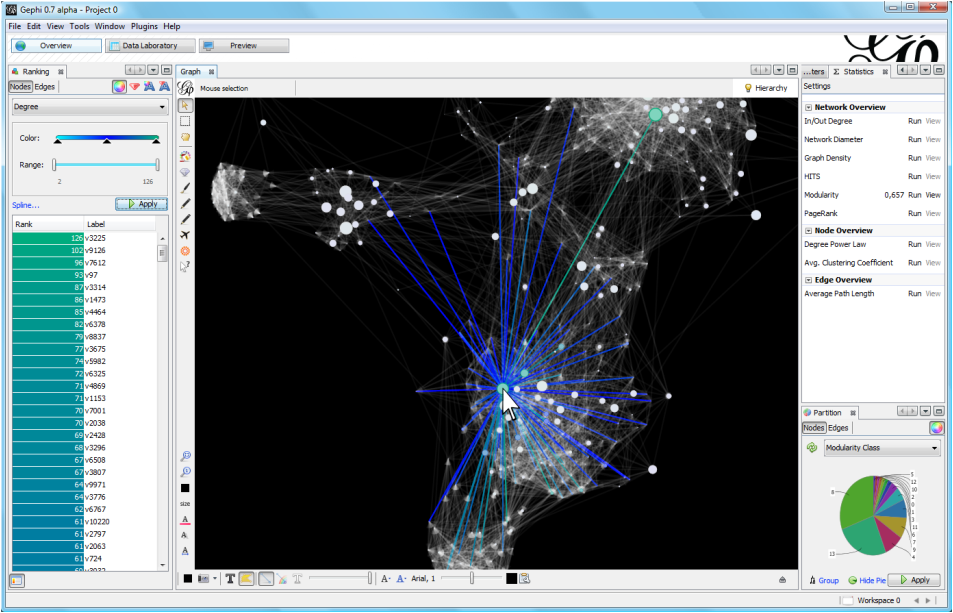
\includegraphics[width=.8\linewidth]{gephi}
\end{figure}

Video: \url{http://youtu.be/6H0veEmTgP0}
\end{frame}

\begin{frame}
\frametitle{Introducci\'on}
\framesubtitle{sigma-js}
\begin{figure}
\centering
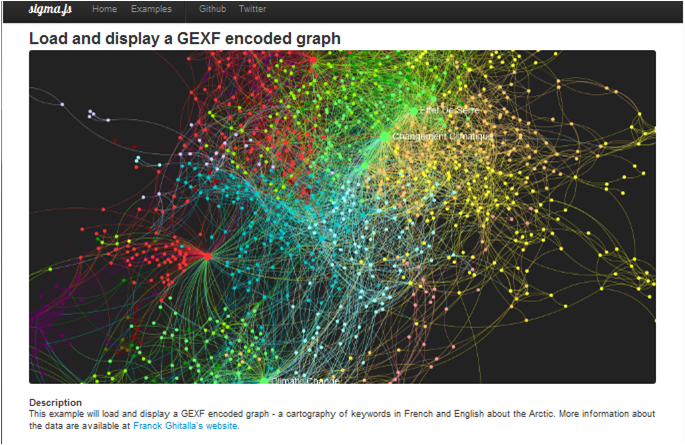
\includegraphics[width=.8\linewidth]{sigmajs}
\end{figure}

Visualizaci\'on: \url{http://sigmajs.org/examples/gexf_example.html}
\end{frame}

\section{C\'omo funciona?: Algunos Ejemplos}
\frame{\frametitle{Agenda}\tableofcontents[currentsection]}


\begin{frame}[fragile]
\frametitle{C\'omo funciona?: Algunos Ejemplos}
\framesubtitle{Ejemplo b\'asico}
\begin{knitrout}\footnotesize
\definecolor{shadecolor}{rgb}{0.969, 0.969, 0.969}\color{fgcolor}\begin{kframe}
\begin{alltt}
\hlfunctioncall{library}(rgexf, quietly = TRUE)
\hlcomment{# Defining a matrix of nodes}
people <- \hlfunctioncall{data.frame}(\hlfunctioncall{matrix}(\hlfunctioncall{c}(1:4, \hlstring{"juan"}, \hlstring{"pedro"}, \hlstring{"matthew"}, \hlstring{"carlos"}), ncol = 2))
\hlcomment{# Defining a matrix of edges}
relations <- \hlfunctioncall{data.frame}(\hlfunctioncall{matrix}(\hlfunctioncall{c}(1, 4, 1, 2, 1, 3, 2, 3, 3, 4, 4, 2, 2, 4, 4, 
    1, 4, 1), ncol = 2, byrow = T))

\hlcomment{# Printing}
\hlfunctioncall{write.gexf}(nodes = people, edges = relations, output = \hlstring{"mygexf.gexf"})
\end{alltt}


{\ttfamily\noindent\itshape\color{messagecolor}{\#\# GEXF graph successfully written at:\\\#\# /home/george/Documents/userrchile/presentaciones/20130615\_paquetes\_en\_\_r/mygexf.gexf}}\end{kframe}
\end{knitrout}

\end{frame}

\begin{frame}[fragile, allowframebreaks=.8]
\frametitle{C\'omo funciona?: Algunos Ejemplos}
\framesubtitle{Ejemplo b\'asico}
\scriptsize
\begin{verbatim}
<?xml version="1.0" encoding="UTF-8"?>
<gexf xmlns="http://www.gexf.net/1.2draft" xmlns:viz="http://www.gexf.net/1.1draft/viz" xmlns:xsi="http://www.w3.org/2001/XMLSchema-instance" xsi:schemaLocation="http://www.gexf.net/1.2draft http://www.gexf.net/1.2draft/gexf.xsd" version="1.2">
  <meta lastmodifieddate="2013-06-15">
    <creator>NodosChile</creator>
    <description>A graph file writing in R using "rgexf"</description>
    <keywords>gexf graph, NodosChile, R, rgexf</keywords>
  </meta>
  <graph mode="static">
    <nodes>
      <node id="1" label="2"/>
      <node id="2" label="4"/>
      <node id="3" label="3"/>
      <node id="4" label="1"/>
    </nodes>
    <edges>
      <edge id="0" source="1" target="4" weight="1.0"/>
      <edge id="1" source="1" target="2" weight="1.0"/>
      <edge id="2" source="1" target="3" weight="1.0"/>
      <edge id="3" source="2" target="3" weight="1.0"/>
      <edge id="4" source="3" target="4" weight="1.0"/>
      <edge id="5" source="4" target="2" weight="1.0"/>
      <edge id="6" source="2" target="4" weight="1.0"/>
      <edge id="7" source="4" target="1" weight="1.0"/>
      <edge id="8" source="4" target="1" weight="1.0"/>
    </edges>
  </graph>
</gexf>
\end{verbatim}
\end{frame}

\section{Algunos hechos (motivantes para nosotros!)}

\frame{\frametitle{Agenda}\tableofcontents[currentsection]}

\begin{frame}
\frametitle{Algunos hechos (motivantes para nosotros!)}
Desde su publicaci\'on hemos recibido consultas desde distintas instituciones/partes del mundo!:
\begin{itemize}[<+->]
\item Prom de 200 descargas mensuales (CRAN)
\item Mismo promedio de visitas mensuales al sitio del proyecto
\item Atenci\'on de investigadores de Universidades (Harvard y Standford por ejemplo)
\item Art\'iculo en el Blog oficial de Gephi
\item Primeros en aparecer en Sitio oficial de GEXF
\item Algunos blogs que han escrito sobre nosotros por ah\'i (\url{http://blogs.msdn.com/b/gpalem/archive/2013/03/29/convert-igraph-r-objects-to-gexf-gephi-format.aspx})
\item Un par de preguntas en Stackoverflow (=D!)
\item ...
\end{itemize}
\end{frame}

\frame{\frametitle{Agenda}\tableofcontents[currentsection]}

\section{Tips para armar paquetes en R}
\begin{frame}
\frametitle{Tips para armar paquetes en R}
\framesubtitle{Cosas que no puedes olvidar}
\begin{itemize}[<+->]
\item Estructura de carpetas ({\tt ?package.skeleton})
\item Todas las funciones (visibles) deben estar documentadas (man)!
\item Todas las Dependencias (a otros paquetes) bien definidas
\item Funciones, m\'etodos y src ``extranjero'' declarados
\item Para su primer paquete ``armen'' uno que ya existe (para probar)
\item (cont.) Mirar codigo ajeno sirve muuucho =P!
\end{itemize}
\end{frame}

\begin{frame}
\frametitle{Tips para armar paquetes en R}
\framesubtitle{{\tt NAMESPACE}}
\begin{figure}
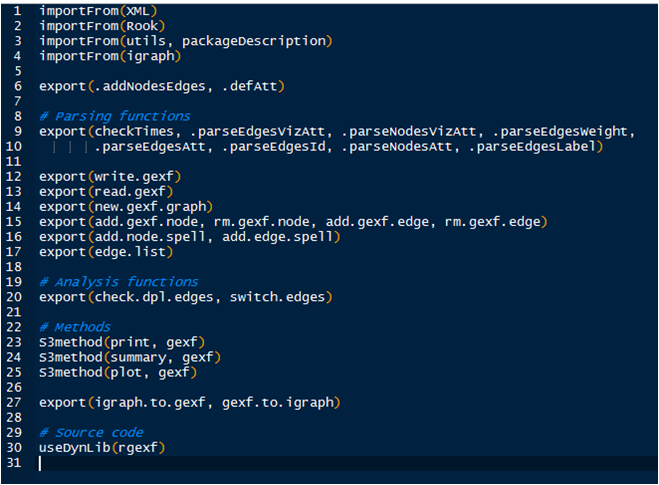
\includegraphics[height=.6\linewidth]{namespace}
\end{figure}
\end{frame}

\begin{frame}
\frametitle{Tips para armar paquetes en R}
\framesubtitle{M\'as tips!}
\begin{itemize}[<+->]
\item Estar atento en la comunidad (revisar Stackoverflow)
\item Mantener actualizado R
\item Utilizar RStudio
A los usuarios les gustan los demos
Instalar {\tt dev\_tools}
\item Utilizar control de versi\'on (Github/google code/bitbucket).
\item Documentar m\'as que bien.
\item Usar carpeta test (no te cuentan mucho pero sirve mucho!).
\item Aprender a usar el archivo .Rbuildignore (o dolor de cabeza).
\item Difundir, difundir difundir (donde importe claro...).
\end{itemize}
\end{frame}

\begin{frame}
\frametitle{Tips para armar paquetes en R}
A los usuarios les gustan los demos... =)
\begin{figure}
\centering
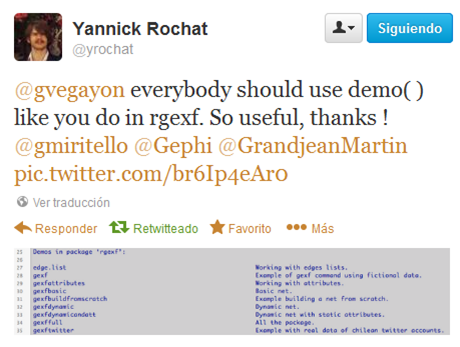
\includegraphics[height=.5\linewidth]{yrochat}
\end{figure}
\end{frame}

\begin{frame}
\frametitle{Tips para armar paquetes en R}
y los paquetes bien documentados...
\begin{figure}
\centering
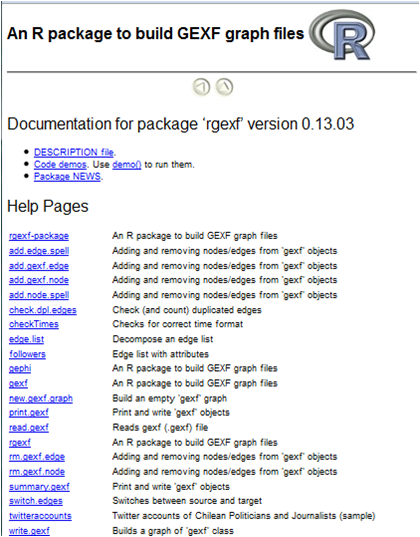
\includegraphics[height=.5\linewidth]{rgexfman}
\end{figure}
\end{frame}

\begin{frame}
\frametitle{Referencias}
\begin{itemize}
\item Sitio web de GEXF \url{http://gexf.net}
\item Sitio web de rgexf \url{https://bitbucket.org/gvegayon/rgexf/}
\item Post de rgexf en el blog de Gephi \url{https://gephi.org/2013/rgexf-an-r-library-to-work-with-gexf-graph-files/}
\item Sitio web sigma-js \url{http://sigmajs.org/}
\item Sitio web de gexf-js \url{https://github.com/raphv/gexf-js}
\item Blog de NodosChile \url{http://www.nodoschile.org/blog/}
\end{itemize}
\end{frame}

\def\title{Gracias!}
\frame{
\maketitle
\begin{centering}
\scriptsize \tt
(presentaci\'on creada en R + knitr + \LaTeX)
\end{centering}
}

\end{document}
